\documentclass[a4paper,12pt]{article}
\usepackage{amsmath,amsthm,amsfonts,amssymb,amscd,amstext,vmargin,graphics,graphicx,tabularx,multicol} 
\usepackage[francais]{babel}
\usepackage[utf8]{inputenc}  
\usepackage[T1]{fontenc} 
\usepackage{pstricks-add,tikz,tkz-tab,variations}
\usepackage[autolanguage,np]{numprint} 

\setmarginsrb{2cm}{1cm}{2cm}{0.5cm}{0cm}{0cm}{0cm}{0cm} %Gauche, haut, droite, haut
\newcounter{numexo}
\newcommand{\exo}[1]{\stepcounter{numexo}\noindent{\bf Exercice~\thenumexo} : \marginpar{\hfill /#1}}
\reversemarginpar


\newcounter{enumtabi}
\newcounter{enumtaba}
\newcommand{\q}{\textbf{\stepcounter{enumtabi} \theenumtabi)}  }
\newcommand{\qa}{\textbf{\stepcounter{enumtaba} (\alph{enumtaba})} }
\newcommand{\initq}{\setcounter{enumtabi}{0}}
\newcommand{\initqa}{\setcounter{enumtaba}{0}}

\newcommand{\be}{\begin{enumerate}}
\newcommand{\ee}{\end{enumerate}}
\newcommand{\bi}{\begin{itemize}}
\newcommand{\ei}{\end{itemize}}
\newcommand{\bp}{\begin{pspicture*}}
\newcommand{\ep}{\end{pspicture*}}
\newcommand{\bt}{\begin{tabular}}
\newcommand{\et}{\end{tabular}}
\renewcommand{\tabularxcolumn}[1]{>{\centering}m{#1}} %(colonne m{} centrée, au lieu de p par défault) 
\newcommand{\tnl}{\tabularnewline}

\newcommand{\bmul}[1]{\begin{multicols}{#1}}
\newcommand{\emul}{\end{multicols}}

\newcommand{\trait}{\noindent \rule{\linewidth}{0.2mm}}
\newcommand{\hs}[1]{\hspace{#1}}
\newcommand{\vs}[1]{\vspace{#1}}

\newcommand{\N}{\mathbb{N}}
\newcommand{\Z}{\mathbb{Z}}
\newcommand{\R}{\mathbb{R}}
\newcommand{\C}{\mathbb{C}}
\newcommand{\Dcal}{\mathcal{D}}
\newcommand{\Ccal}{\mathcal{C}}
\newcommand{\mc}{\mathcal}

\newcommand{\vect}[1]{\overrightarrow{#1}}
\newcommand{\ds}{\displaystyle}
\newcommand{\eq}{\quad \Leftrightarrow \quad}
\newcommand{\vecti}{\vec{\imath}}
\newcommand{\vectj}{\vec{\jmath}}
\newcommand{\Oij}{(O;\vec{\imath}, \vec{\jmath})}
\newcommand{\OIJ}{(O;I,J)}


\newcommand{\reponse}[1][1]{%
\multido{}{#1}{\makebox[\linewidth]{\rule[0pt]{0pt}{20pt}\dotfill}
}}

\newcommand{\titre}[5] 
% #1: titre #2: haut gauche #3: bas gauche #4: haut droite #5: bas droite
{
\noindent #2 \hfill #4 \\
#3 \hfill #5

\vspace{-1.6cm}

\begin{center}\rule{6cm}{0.5mm}\end{center}
\vspace{0.2cm}
\begin{center}{\large{\textbf{#1}}}\end{center}
\begin{center}\rule{6cm}{0.5mm}\end{center}
}



\begin{document}
\pagestyle{empty}
\titre{Contrôle 4 : Coordonées d'un point du plan }{Nom :}{Prénom :}{\textbf{2nd 8}}{Date:}


\vspace*{0.5cm}
\exo{7.5} Cours\\

\initq \q Soient  A(2 ; 5) et B(3 ; 9) deux points du plan muni d'un repère orthonormé.\\
Calculer les coordonnées du point M milieu de [AB].\\

\q Soient  A(3 ; 7) et B(4 ; 10) deux points du plan muni d'un repère orthonormé.\\
Calculer la distance AB.\\

\q Soient  A(2 ; 1), B(4 ; -3) et C(-2 ; -1) trois points du plan muni d'un repère orthonormé.\\
Quelle est la nature du triangle ABC ? Justifier votre réponse.\\



\vspace*{0.5cm}

\exo{3}

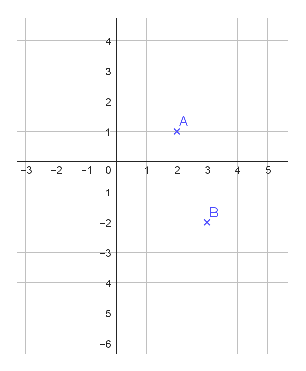
\includegraphics[scale=1.7]{grillecontrole2.eps} 

\initq \q Lire les coordonnées des points A et B.\\

\q Placer le point N, symétrique du point B par rapport au point A.\\ Donner les coordonnées du point N.\\



\vspace*{0.5cm}

\exo{5.5}\\
Pour chaque affirmation suivante, dire si elle est vraie ou fausse. Justifier votre réponse.\\
On considère les points A(1 ; 2), B(-2 ; -1), C(4 ; 5), D(-1 ; 3), E(2 ; 1) et F(3 ; 1).\\
\initq \q BDCE est un parallélogramme.\\
\q Le point F est le symétrique du point D par rapport à A.\\
\q Le point C appartient au cercle de centre A et de rayon 5.\\



\vspace*{0.5cm}

\exo{4}
On considère les points A(-2 ; 3), B(2 ; 4), C(4 ; 2).\\
Calculer les coordonnées du point D tel que ABCD soit un parallélogramme.\\

\end{document}
